% !TEX program = xelatex
% Статья для сборника НИТУ «МИСиС».
% Шаблон: sadekovlar/misis-article-latex (XeLaTeX, две колонки).
% Сборка: make article  →  build/article.pdf

\documentclass{misisarticle}

% Кириллический шрифт, метрически совместимый с Times New Roman.
% Файлы лежат в fonts/, поэтому сборка не зависит от набора шрифтов системы.
\setmainfont{LiberationSerif}[
  Path=./fonts/, Extension=.ttf,
  UprightFont=*-Regular, BoldFont=*-Bold,
  ItalicFont=*-Italic, BoldItalicFont=*-BoldItalic,
  Ligatures=TeX,
]
\renewfontfamily\cyrillicfont{LiberationSerif}[
  Path=./fonts/, Extension=.ttf,
  UprightFont=*-Regular, BoldFont=*-Bold,
  ItalicFont=*-Italic, BoldItalicFont=*-BoldItalic,
  Ligatures=TeX,
]
\renewfontfamily\cyrillicfontsf{LiberationSerif}[
  Path=./fonts/, Extension=.ttf,
  UprightFont=*-Regular, BoldFont=*-Bold,
  ItalicFont=*-Italic, BoldItalicFont=*-BoldItalic,
]
\renewfontfamily\cyrillicfonttt{LiberationMono}[
  Path=./fonts/, Extension=.ttf, UprightFont=*-Regular,
]

\usepackage{amsmath}
\usepackage{booktabs}
\usepackage{float}

% ---------- классификаторы ----------
\grnti{28.23.15, 27.41.17}
\asjc{1702, 2207}
\oecd{1.02, 2.02}

% ---------- заголовок ----------
\title{Восстановление ориентации и траектории кисти по данным акселерометра и гироскопа смартфона с коррекцией дрейфа по остановкам}

% ---------- авторы ----------
\misisauthor{Н.~В.~Запольских}{кафедра инженерной кибернетики НИТУ «МИСиС»}{Москва, Россия}{m2300593@edu.misis.ru}

% ---------- аннотация ----------
\abstract{%
  Рассматривается восстановление ориентации и траектории кисти по показаниям акселерометра и гироскопа смартфона. Положение нельзя измерить напрямую: ускорение интегрируется дважды, поэтому смещение нуля и ошибка наклона быстро накапливаются. Описан конвейер из калибровки по шести положениям, расширенного фильтра Калмана с гейтом акселерометра, детектора остановок и коррекции постоянной ошибки ускорения на участках «покой--покой». Коррекция оценивает постоянную составляющую из условия нулевого интеграла скорости между остановками и переинтегрирует участок, не меняя форму движения. На синтетической записи длительностью 60~с ошибка ориентации в модели составила $1{,}48^\circ$, в приложении~--- $2{,}34^\circ$, а RMSE положения в приложении~--- 0,59~м; после коррекции RMSE уменьшился до 0,27~м. На реальной записи UCI~HAR детектор отнёс к покою 97,2\,\% отсчётов и не дал ложных срабатываний при ходьбе. На собственных записях смартфона итоговое смещение при покачивании в одной точке уменьшилось с 1,423 до 0,071~м и с 0,188 до 0,037~м. Результат показывает, что на коротких записях главная причина ухода~--- почти постоянная ошибка ускорения, а не случайный шум.
}

\keywords{%
  инерциальные датчики, оценка ориентации, кватернион, фильтр Калмана, ZUPT, коррекция дрейфа
}

\hypersetup{%
  pdftitle={Восстановление ориентации и траектории кисти по данным акселерометра и гироскопа смартфона с коррекцией дрейфа по остановкам},
  pdfauthor={Н. В. Запольских},
  pdfkeywords={инерциальные датчики, оценка ориентации, кватернион, фильтр Калмана, ZUPT, коррекция дрейфа},
}

\begin{document}

\maketitle

% ============================================================
\section{Введение}

Акселерометр и гироскоп есть почти в каждом смартфоне. Они не требуют камер, маркеров и оборудованной комнаты, поэтому смартфон удобно использовать для записи движения руки: в реабилитации, спорте, робототехнике и компьютерных играх. Главная трудность состоит в том, что положение не измеряется напрямую. Акселерометр показывает ускорение, и чтобы получить координаты, его нужно дважды проинтегрировать. Любая небольшая ошибка при этом накапливается: при постоянной ошибке ускорения $0{,}01$~м/с$^2$ ошибка положения через 10~с составляет около 0,5~м, а через минуту~--- десятки метров~\cite{woodman}.

Оптические системы с маркерами точны, но требуют нескольких камер и прямой видимости. Механические перчатки измеряют углы пальцев, но стесняют руку и не дают положения кисти. Инерциальный модуль автономен и компактен, однако его показания нужно калибровать, фильтровать и ограничивать накопление ошибки~\cite{kortier,shenoy}.

Цель работы~--- собрать и проверить на одном смартфоне полный конвейер, который оценивает ориентацию кисти и восстанавливает траекторию с ошибкой в несколько сантиметров на коротких записях. Отдельно исследуется, какая составляющая ошибки определяет уход траектории при движении с остановками.

Новизна работы не в отдельных алгоритмах: кватернионы, фильтр Калмана и обнуление скорости известны. Вклад состоит в трёх вещах. Собран воспроизводимый конвейер «калибровка--ориентация--детектор остановок--интегрирование--коррекция», работающий на смартфоне в реальном времени. Предложена и проверена коррекция по остановкам: на каждом участке «покой--покой» из ускорения вычитается постоянная составляющая, найденная из условия нулевого интеграла скорости. На одной и той же синтетической записи количественно сравнены интегрирование гироскопа, комплементарный фильтр и расширенный фильтр Калмана, а итоговый конвейер проверен на открытой записи UCI~HAR и двух собственных записях.

% ============================================================
\section{Анализ работ}

\subsection{Системы отслеживания кисти}

В работе~\cite{kortier} инерциальные и магнитные датчики закреплены на кисти, пальцах и большом пальце. Система восстанавливает все суставы; ошибка положения кончика пальца относительно оптической системы составила $5\pm0{,}5$~мм при сгибании и $12{,}4\pm3{,}0$~мм при комбинированном движении. В~\cite{shenoy} собрана система из 16 модулей BNO055, которая передаёт ориентацию на частоте 100~Гц; точность признана приемлемой для лабораторных измерений, но надевать систему долго. В~\cite{pellois} инерциальные датчики применены для трекинга руки в роботизированной среде, а в~\cite{miyazaki} исследован трекинг кисти по одному модулю и получена приблизительная оценка без подтверждённой абсолютной точности.

Общий вывод простой: высокая точность достигается либо многими датчиками, либо внешней опорой. Решение на одном смартфоне оценивает только движение кисти как твёрдого тела, зато не требует специальной подготовки.

\subsection{Дрейф и обнуление скорости}

В работе~\cite{neto} для операции «взять предмет и поставить его» интегрирование выполнялось только во время движения, а в остановках скорость обнулялась. Ошибка в горизонтальной плоскости составила около 1~см. Этот приём известен как ZUPT (zero velocity update). В~\cite{niu} малые перемещения восстанавливаются по одному МЭМС-акселерометру с компенсацией медленного тренда.

ZUPT ограничивает накопление ошибки, но не убирает её причину. Если между двумя остановками интеграл ускорения не равен нулю, траектория успевает уйти в сторону, а после остановки остаётся смещённой. Именно этот остаток исследуется в настоящей работе.

\subsection{Ориентация и калибровка}

Комплементарный фильтр на группе вращений описан в~\cite{mahony}: он смешивает быстрое интегрирование гироскопа с медленной поправкой по направлению силы тяжести. Кватернионное описание ориентации и построение жестов по инерциальным модулям рассмотрены в~\cite{zhilin}. Расширенный фильтр Калмана (EKF) дополнительно хранит ковариацию ошибки и сам выбирает степень доверия к акселерометру.

Калибровка МЭМС-датчиков обычно выполняется по известным положениям. В~\cite{tedaldi} модуль вручную ставят в 37 положений и по показаниям силы тяжести находят масштабы, перекосы и смещения. В~\cite{zhang} использован поворотный стенд и показано, что раздельная калибровка датчиков не гарантирует согласования их осей. В~\cite{batista} смещение акселерометра и направление гравитации оцениваются фильтром Калмана. Для смартфона полная калибровка по 37 положениям неудобна: пользователь не знает точных углов. Поэтому в работе используется компромисс~--- шесть положений по осям.

\subsection{Работы кафедры и преподавателя}

В сборнике кафедры~\cite{epifanov} исследуются алгоритмы замыкания цикла в лидарной одометрии: накопленный дрейф корректируется по ранее посещённым местам. В~\cite{vershinin} рассматривается непрерывное распознавание языка жестов по видео: положение ключевых точек руки и последовательность жестов. Обе работы близки к задаче оценки движения, но опираются на внешние сенсоры~--- лидар и камеру. Работа~\cite{kataev} оценивает параметры ходьбы человека по двум акселерометрам и показывает, как инерциальные данные дают количественные характеристики движения без внешних камер.

Наша задача дополняет эти направления с другой стороны: абсолютной привязки нет, зато система автономна и использует только датчики, уже установленные в телефоне. Совместной проверки на одном смартфоне полного конвейера с калибровкой по шести положениям, гейтом акселерометра, ZUPT и коррекцией постоянной ошибки между остановками в рассмотренных работах нет.

% ============================================================
\section{Постановка задачи}

Заданы множество моментов времени $T=\{t_0,\dots,t_N\}$ с шагом $\Delta t$, множество измерений акселерометра $A=\{\mathbf a_0,\dots,\mathbf a_N\}$ и гироскопа $\Omega=\{\boldsymbol\omega_0,\dots,\boldsymbol\omega_N\}$, $\mathbf a_k,\boldsymbol\omega_k\in\mathbb R^3$. Требуется найти множества ориентаций $Q=\{\mathbf q_0,\dots,\mathbf q_N\}$, скоростей $V=\{\mathbf v_0,\dots,\mathbf v_N\}$ и положений $P=\{\mathbf p_0,\dots,\mathbf p_N\}$.

Измерения связаны с истинными величинами моделью
\begin{equation}
\tilde{\mathbf a}_k=\mathbf M_a\mathbf a_k+\mathbf b_a+\boldsymbol\eta_{a,k},\qquad
\tilde{\boldsymbol\omega}_k=\mathbf M_g\boldsymbol\omega_k+\mathbf b_g+\boldsymbol\eta_{g,k},
\label{eq:model}
\end{equation}
где $\mathbf M_a,\mathbf M_g$~--- матрицы масштабов и перекосов осей; $\mathbf b_a,\mathbf b_g$~--- смещения нуля; $\boldsymbol\eta_{a,k},\boldsymbol\eta_{g,k}$~--- шумы.

Ориентация хранится кватернионом $\mathbf q=(q_0,q_1,q_2,q_3)$ с условием $\|\mathbf q\|=1$. Кватернион не имеет вырождения, которое возникает у углов Эйлера~\cite{zhilin}. Ориентация обновляется по угловой скорости:
\begin{equation}
\mathbf q_k=\mathbf q_{k-1}\otimes\exp\!\left(\tfrac12\boldsymbol\omega_k\Delta t\right),
\label{eq:quat}
\end{equation}
где $\otimes$~--- умножение кватернионов. Матрица поворота $\mathbf R(\mathbf q)$ переводит показания в навигационную систему. Линейное ускорение получается после вычитания гравитации:
\begin{equation}
\mathbf a_k^{n}=\mathbf R(\mathbf q_k)\tilde{\mathbf a}_k-\mathbf g,\qquad \mathbf g=(0,0,9{,}81)^\mathrm T.
\label{eq:lin}
\end{equation}
Скорость и положение находятся методом трапеций:
\begin{align}
\mathbf v_k&=\mathbf v_{k-1}+\tfrac{\Delta t}{2}\left(\mathbf a_k^{n}+\mathbf a_{k-1}^{n}\right),
\label{eq:v}\\
\mathbf p_k&=\mathbf p_{k-1}+\tfrac{\Delta t}{2}\left(\mathbf v_k+\mathbf v_{k-1}\right).
\label{eq:p}
\end{align}

Для обнаружения остановки вычисляется дисперсия модуля ускорения в окне из $n$ отсчётов:
\begin{equation}
\sigma_k^2=\frac{1}{n-1}\sum_{j=k-n+1}^{k}\left(\|\mathbf a_j\|-\overline{\|\mathbf a\|}\right)^2.
\label{eq:var}
\end{equation}
Признак остановки равен единице, если одновременно $\sigma_k^2<\lambda_a^2$ и $\|\boldsymbol\omega_k\|<\lambda_\omega$; иначе он равен нулю. В покое скорость обнуляется: $\mathbf v_k=\mathbf 0$, $\mathbf p_k=\mathbf p_{k-1}$.

Качество решения оценивается средней квадратичной ошибкой
\begin{equation}
\mathrm{RMSE}=\sqrt{\frac{1}{N+1}\sum_{k=0}^{N}\|\tilde{\mathbf p}_k-\mathbf p_k\|^2}
\label{eq:rmse}
\end{equation}
и ошибкой в последний момент $e_{\text{end}}=\|\tilde{\mathbf p}_N-\mathbf p_N\|$, где $\tilde{\mathbf p}_k$~--- найденное положение, $\mathbf p_k$~--- истинное.

Коротко постановку можно записать так. \textbf{Дано:} $T$, $A$, $\Omega$, $\Delta t$, $\mathbf g$, параметры калибровки $\mathbf M_a,\mathbf b_a,\mathbf b_g$, пороги $\lambda_a,\lambda_\omega$, размер окна $n$. \textbf{Найти:} $Q$, $V$, $P$. \textbf{Условия:} уравнения~\eqref{eq:model}--\eqref{eq:p}; все кватернионы единичные; признак остановки принимает значения 0 или 1; при остановке скорость равна нулю. \textbf{Критерий:} минимизировать ошибку~\eqref{eq:rmse} при ограничении на $e_{\text{end}}$.

% ============================================================
\section{Описание метода}

Схема обработки показана на рис.~\ref{fig:pipeline}. Все операции~--- арифметика с векторами и матрицами размера $3\times3$, поэтому конвейер работает на смартфоне в реальном времени.

\begin{figure}[htbp]
  \centering
  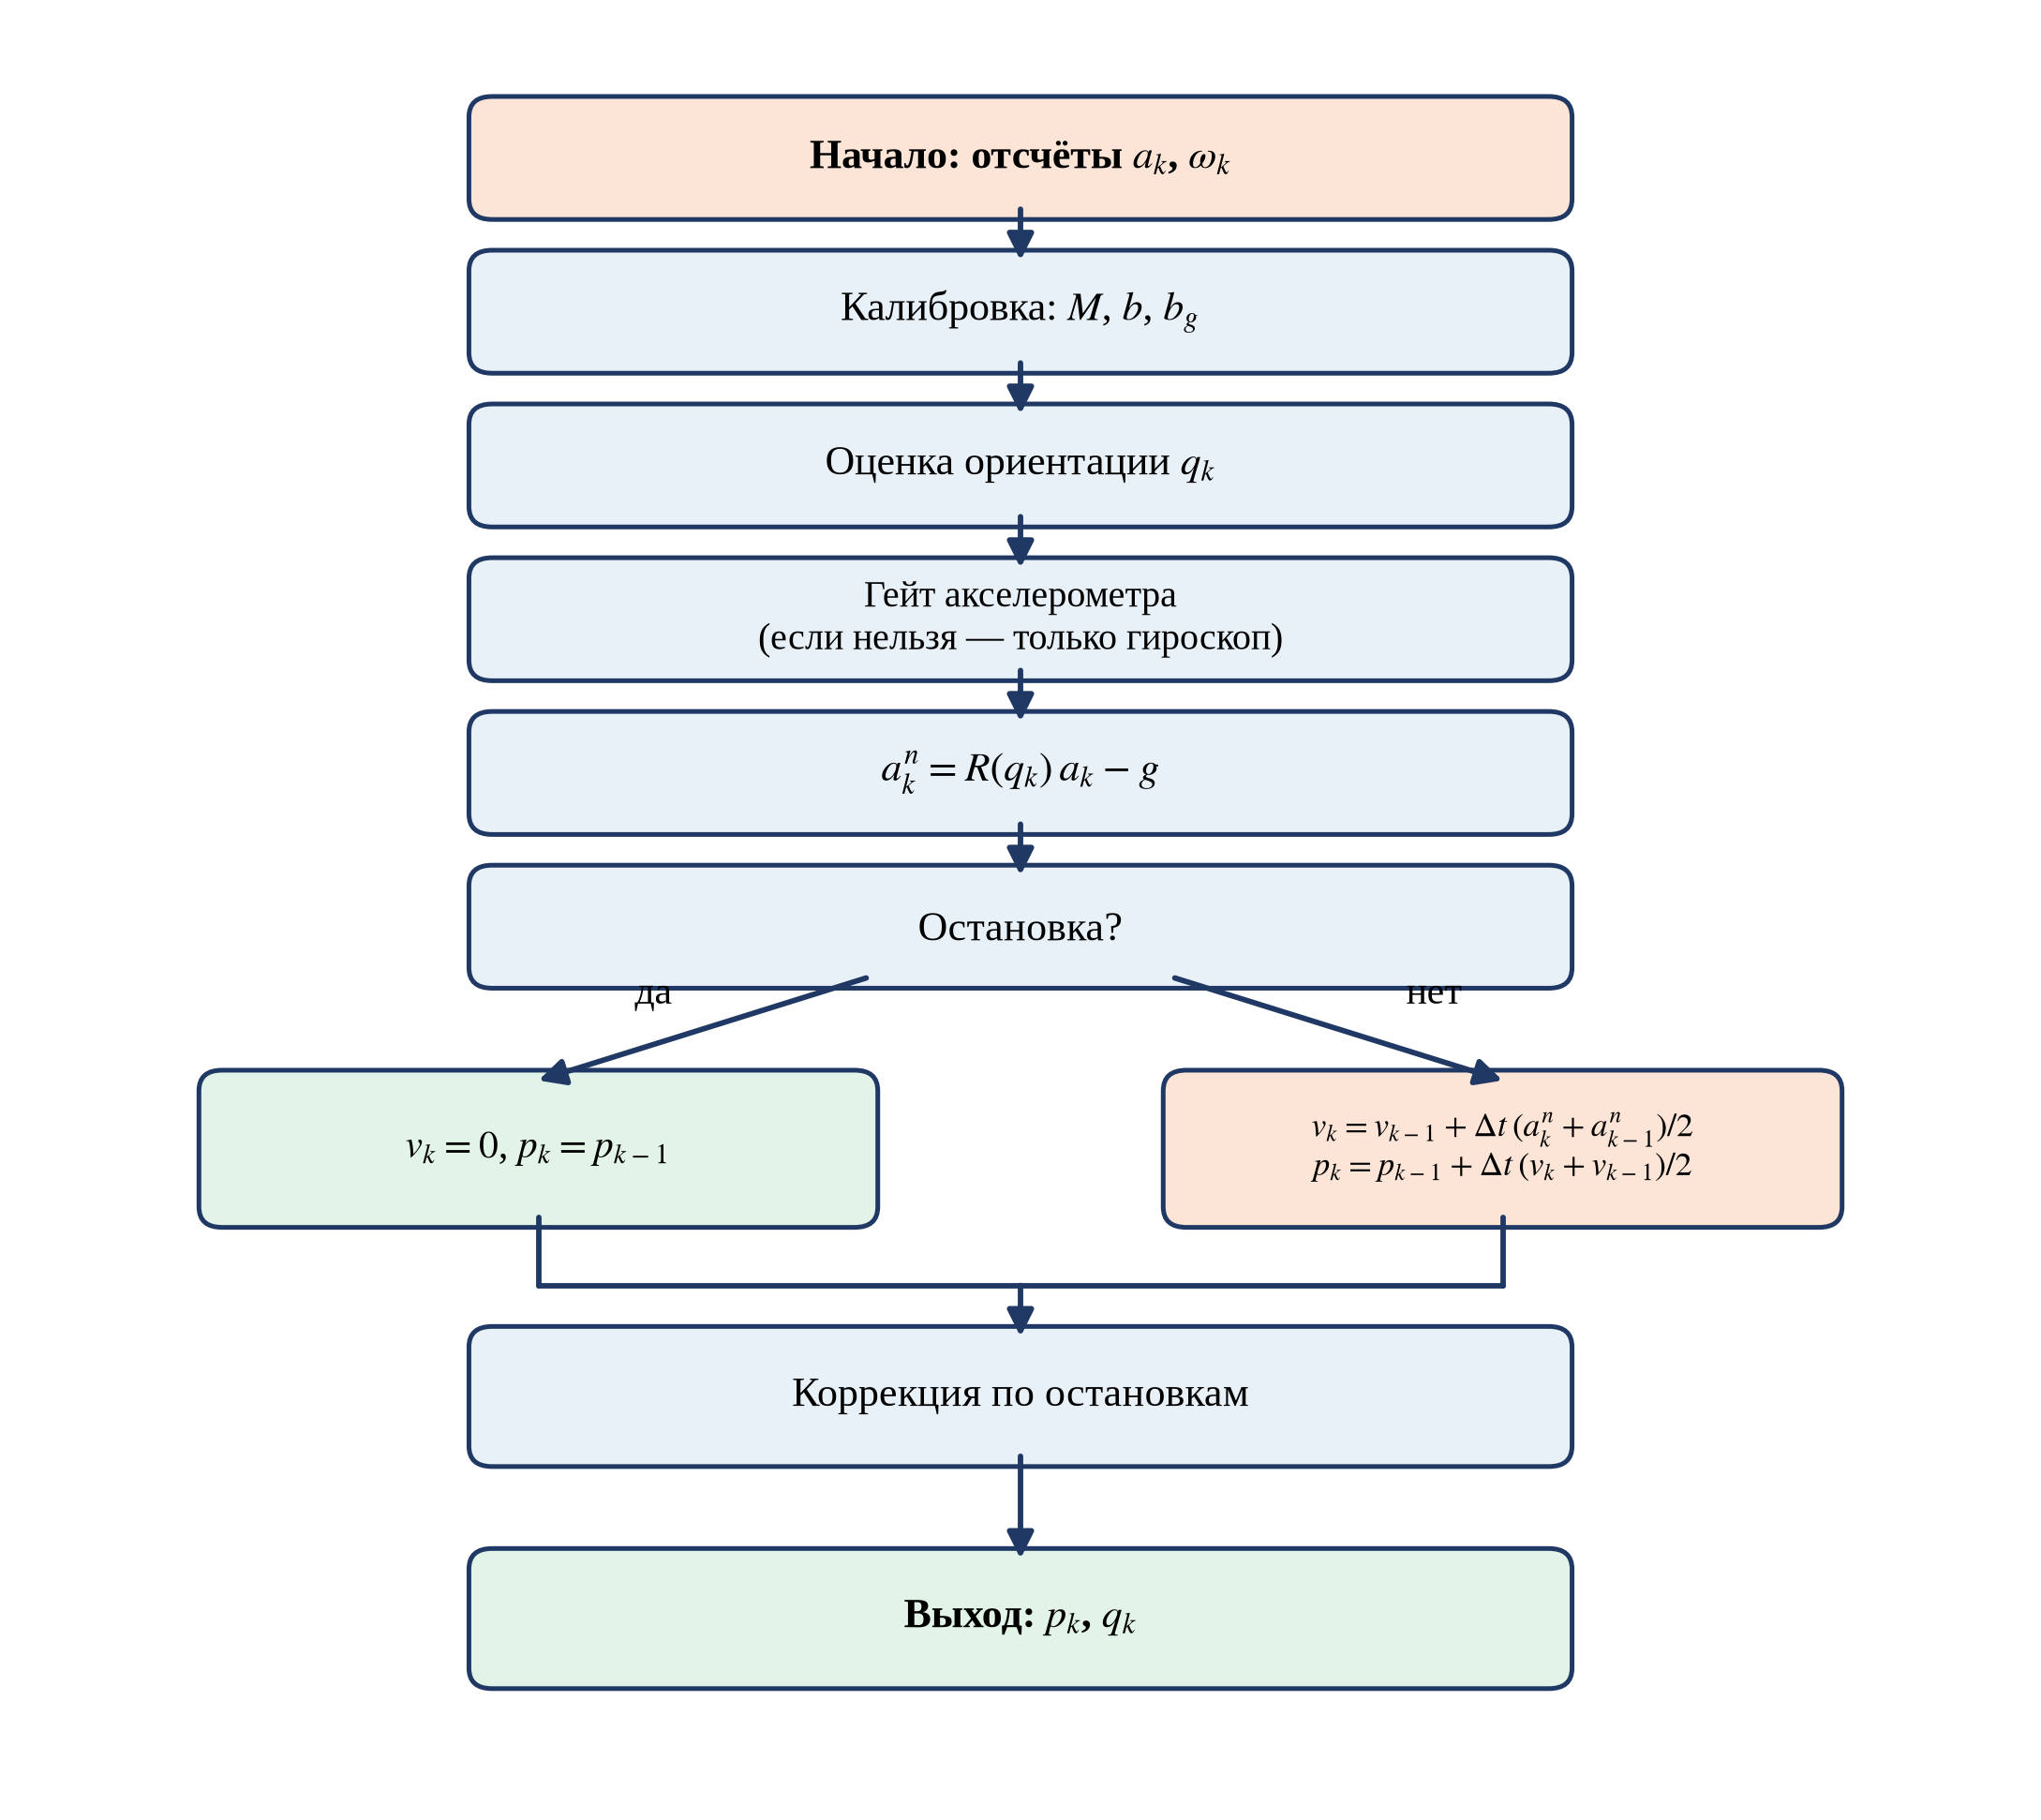
\includegraphics[width=\columnwidth]{figures/fig1_pipeline.png}
  \caption{Схема обработки: калибровка, оценка ориентации, вычитание гравитации, детектор остановок, интегрирование и коррекция по остановкам}
  \label{fig:pipeline}
\end{figure}

\subsection{Калибровка}

Пока телефон неподвижен, акселерометр измеряет только реакцию на гравитацию, а гироскоп~--- только смещение нуля. Смещение гироскопа оценивается средним по 1,5~с покоя. Калибровка акселерометра выполняется по шести положениям: $Z^-$, $Y^+$, $X^+$, $Y^-$, $X^-$, $Z^+$. В каждом положении телефон держат неподвижно 2~с, а приложение проверяет, что отклонение нужной оси от гравитации не больше $2^\circ$.

Для каждой оси используются два противоположных положения. Смещение и столбец матрицы находятся как
\begin{equation}
\mathbf b=\frac{\mathbf a_p+\mathbf a_m}{2},\qquad
\mathbf m_i=\frac{\mathbf a_p-\mathbf a_m}{2g},
\label{eq:calib}
\end{equation}
где $\mathbf a_p,\mathbf a_m$~--- средние показания в положениях с положительным и отрицательным направлением оси; $\mathbf m_i$~--- соответствующий столбец $\mathbf M_a$; $g=9{,}81$~м/с$^2$. После калибровки показания пересчитываются по формуле $\mathbf a=\mathbf M_a^{-1}(\tilde{\mathbf a}-\mathbf b)$. Качество проверяется по остаточной ошибке: при остатке меньше 0,03~м/с$^2$ и масштабах в пределах 0,97--1,03 калибровка считается хорошей, при остатке меньше 0,06~м/с$^2$~--- приемлемой. Плохая калибровка не применяется.

Такой способ уступает полной калибровке по 37 положениям~\cite{tedaldi}, но занимает около минуты и понятен пользователю. Он учитывает не только смещение, но и масштаб с перекосами осей.

\subsection{Оценка ориентации}

Ориентация оценивается расширенным фильтром Калмана. Состояние~--- малый поворот, то есть ошибка ориентации; прогноз делается по гироскопу, коррекция~--- по направлению силы тяжести. Матрица ковариации хранит, насколько оценка неточна. Если измерения шумные, фильтр больше доверяет модели, если модель неточная~--- сильнее подправляется по измерениям.

При вращении акселерометр измеряет не только гравитацию, но и центростремительное и тангенциальное ускорение. Принимать их за наклон нельзя. Поэтому перед коррекцией проверяется гейт:
\begin{equation}
\left(\|\mathbf a_k\|-g\right)^2>\lambda_{\text{gate}}^2
\quad\text{или}\quad
\|\boldsymbol\omega_k\|>\lambda_{\omega,\text{gate}}.
\label{eq:gate}
\end{equation}
Если условие выполнено, поправка по акселерометру пропускается, и ориентация обновляется только гироскопом. В работе приняты $\lambda_{\text{gate}}=0{,}35$~м/с$^2$ и $\lambda_{\omega,\text{gate}}=0{,}6$~рад/с. В покое акселерометр считается надёжнее, поэтому поправка усиливается (ZARU). Для сравнения использованы чистое интегрирование гироскопа и комплементарный фильтр~\cite{mahony}.

\subsection{Детектор остановок и коррекция по остановкам}

Детектор сравнивает дисперсию~\eqref{eq:var} с порогом и проверяет модуль угловой скорости. В покое дисперсия падает на два--три порядка, поэтому остановка видна отчётливо. Размер окна выбран 25 отсчётов: при 100~Гц это 0,25~с, что меньше длительности обычной остановки. Пороги $\lambda_a=0{,}12$~м/с$^2$ и $\lambda_\omega=0{,}10$~рад/с получены на синтетической записи и затем проверены на реальной. Решение принимается только при выполнении обоих условий: одно условие по ускорению может сработать при равномерном движении, одно по угловой скорости~--- при медленном повороте.

На участке между двумя остановками скорость в начале и в конце равна нулю. Поэтому интеграл линейного ускорения по участку должен быть нулевым. На практике из-за смещения акселерометра, ошибки масштаба и остатка гравитации он не равен нулю; этот остаток и даёт линейный уход траектории. Пусть участок начинается в момент $t_0$ и заканчивается в $t_1$. Приращение скорости по методу трапеций равно
\begin{equation}
\Delta\mathbf v=\sum_{k}\frac{\Delta t_k}{2}\left(\mathbf a_k^{n}+\mathbf a_{k-1}^{n}\right).
\label{eq:dv}
\end{equation}
Постоянная ошибка оценивается как
\begin{equation}
\mathbf c=\frac{\Delta\mathbf v}{T-\Delta t_1/2},
\label{eq:corr}
\end{equation}
где $T=t_1-t_0$~--- длительность участка, $\Delta t_1$~--- первый шаг участка. Затем $\mathbf c$ вычитается из линейного ускорения на всём участке, и участок переинтегрируется. На остановке скорость снова обнуляется, а положение фиксируется.

Форма движения при этом сохраняется: убирается только постоянная составляющая, которая не может быть настоящим ускорением при движении от покоя до покоя. Коррекция применяется только к участкам, ограниченным двумя достаточно длинными остановками; ведущие и завершающие участки без опоры не трогаются. Сырые данные не изменяются: исправляется только траектория, а параметры коррекции сохраняются в метаданных сессии.

\subsection{Реализация}

Синтетическая модель и первичные расчёты выполнены на Python. Итоговое приложение написано на Kotlin с использованием Jetpack Compose и собрано через Gradle. Математика не зависит от Android: модули \texttt{OrientationEkf}, \texttt{ZuptDetector}, \texttt{TrajectoryIntegrator}, \texttt{RestSegmentCorrector} и \texttt{StreamingTracker} вынесены в отдельный модуль. Приложение подписывается на акселерометр и гироскоп через системный менеджер датчиков, хранит сырые показания в CSV и сохраняет сессию в отдельную папку: \texttt{raw.csv}, \texttt{trajectory.csv}, \texttt{meta.json}, \texttt{log.txt} и снимок траектории. Запись идёт через MediaStore, поэтому разрешения на доступ к файлам не нужны.

% ============================================================
\section{Эксперименты и результаты}

\subsection{Синтетическая запись}

Синтетическая запись имитировала перенос предмета: три участка движения длительностью около 2~с чередовались с остановками по 1,5~с. Общая длительность~--- 60~с, частота~--- 100~Гц, число отсчётов~--- 6000. В показания добавлялись смещение акселерометра $(0{,}010;-0{,}008;0{,}006)$~м/с$^2$, шум 0,05~м/с$^2$, смещение гироскопа $(1{,}0;-0{,}7;0{,}4)^\circ$/с, шум 0,05~$^\circ$/с и медленное случайное изменение смещения 0,03~$^\circ$/(с$\cdot\sqrt{\text{с}}$).

Сначала сравнивались три способа оценки ориентации на одной и той же записи (табл.~\ref{tab:orient}). Комплементарный фильтр проиграл потому, что при движении принимал линейное ускорение за наклон и вносил неверную поправку. Фильтр Калмана учитывает, насколько сильно показания ускорения отличаются от силы тяжести, и поэтому ошибается меньше.

\begin{table}[H]
  \caption{Ошибка ориентации на синтетической записи}
  \label{tab:orient}
  \centering
  \footnotesize
  \begin{tabular}{lcc}
    \toprule
    Способ & RMSE, $^\circ$ & Ошибка в конце, $^\circ$ \\
    \midrule
    Интегрирование гироскопа & 3,74 & 6,34 \\
    Комплементарный фильтр & 12,77 & 24,03 \\
    Фильтр Калмана & 1,48 & 0,49 \\
    \bottomrule
  \end{tabular}
\end{table}

Ошибка положения приведена в табл.~\ref{tab:pos}. Даже при идеальной ориентации ошибка за минуту достигает 23,6~м: сказывается смещение акселерометра. Совместная работа фильтра и детектора остановок уменьшила ошибку за 60~с примерно в 20 раз, а коррекция по остановкам~--- ещё в два раза.

\begin{table}[H]
  \caption{Ошибка положения на синтетической записи, м}
  \label{tab:pos}
  \centering
  \footnotesize
  \setlength{\tabcolsep}{3pt}
  \begin{tabular}{lcccc}
    \toprule
    Вариант & RMSE & Макс. & RMSE & Макс. \\
     & 60~с & 60~с & 12~с & 12~с \\
    \midrule
    Идеальная ориентация & 10,51 & 23,62 & 0,42 & 0,95 \\
    Комплементарный фильтр & 317,56 & 712,47 & 9,67 & 23,35 \\
    Фильтр Калмана & 16,79 & 42,16 & 0,33 & 0,75 \\
    Фильтр Калмана + ZUPT & 0,83 & 1,53 & 0,08 & 0,12 \\
    Приложение (EKF + ZUPT) & 0,59 & 0,88 & 0,11 & 0,24 \\
    Приложение + коррекция & 0,27 & 0,42 & 0,08 & 0,16 \\
    \bottomrule
  \end{tabular}
\end{table}

\subsection{Реальная запись UCI HAR}

В наборе UCI~HAR~\cite{uci} частота записи~--- 50~Гц, одно окно длится 2,56~с. Для первого испытуемого взято 95 окон ходьбы. Среднее квадратичное отклонение модуля ускорения при ходьбе составило 0,245~$g$, а в покое~--- 0,0025~$g$, то есть почти в сто раз меньше. Средний модуль угловой скорости в покое~--- 0,034~рад/с; это остаточное смещение нуля и шум.

Детектор остановок не дал ни одного ложного срабатывания при ходьбе, а в состоянии стояния отнёс к покою 97,2\,\% отсчётов. Остальные 2,8\,\% приходятся на начало окна, когда статистика ещё не набралась. Значит, настройки, полученные на синтетике, подходят и для реальных сигналов. Оценка перемещения за одно окно ходьбы дала около 1,16~м при максимальной скорости 0,96~м/с. Это ориентировочная величина: истинной траектории в наборе нет, а датчик закреплён на поясе, но порядок величины соответствует шагу человека.

\subsection{Собственные записи}

Проверка выполнена на смартфоне INFINIX X676C (Android~12). Перед записью телефон лежал неподвижно: приложение оценивало смещение гироскопа за 1,5~с. Калибровка акселерометра по шести положениям была выполнена заранее и сохранена в памяти телефона.

Первая серия проверяла главную проблему~--- уход траектории при покачивании телефона в одной точке. Телефон лежал на столе, его покачивали вокруг оси $X$, затем останавливали, после чего покачивали вокруг оси $Y$. Постороннего перемещения не было, поэтому истинное смещение должно быть близко к нулю. Запись длилась 19,0~с, частота~--- 107,1~Гц, число точек траектории~--- 2012.

На этой записи версия 0.3.0 показала итоговое смещение 1,423~м. Причина~--- почти постоянная ошибка ускорения на участках движения: 0,038 и 0,048~м/с$^2$. После коррекции по остановкам на тех же данных осталось 0,071~м. После доработки была сделана вторая запись: 9,84~с, 1042 точки, частота 105,6~Гц, два покачивания с остановками. В версии 0.3.1 приложение автоматически исправило два участка: итоговое смещение уменьшилось с 0,188 до 0,037~м, а смещение после первой остановки~--- с 0,089 до 0,016~м. Результаты сведены в табл.~\ref{tab:real} и показаны на рис.~\ref{fig:real}.

\begin{table}[H]
  \caption{Результаты на собственных записях}
  \label{tab:real}
  \centering
  \footnotesize
  \setlength{\tabcolsep}{4pt}
  \begin{tabular}{lcccc}
    \toprule
    Сессия & Версия & $t$, с & До, м & После, м \\
    \midrule
    Покачивание $X$, затем $Y$ & 0.3.0 & 19,00 & 1,423 & 0,071 \\
    Покачивание $X$, затем $Y$ & 0.3.1 & 9,84 & 0,188 & 0,037 \\
    \bottomrule
  \end{tabular}
\end{table}

\begin{figure}[htbp]
  \centering
  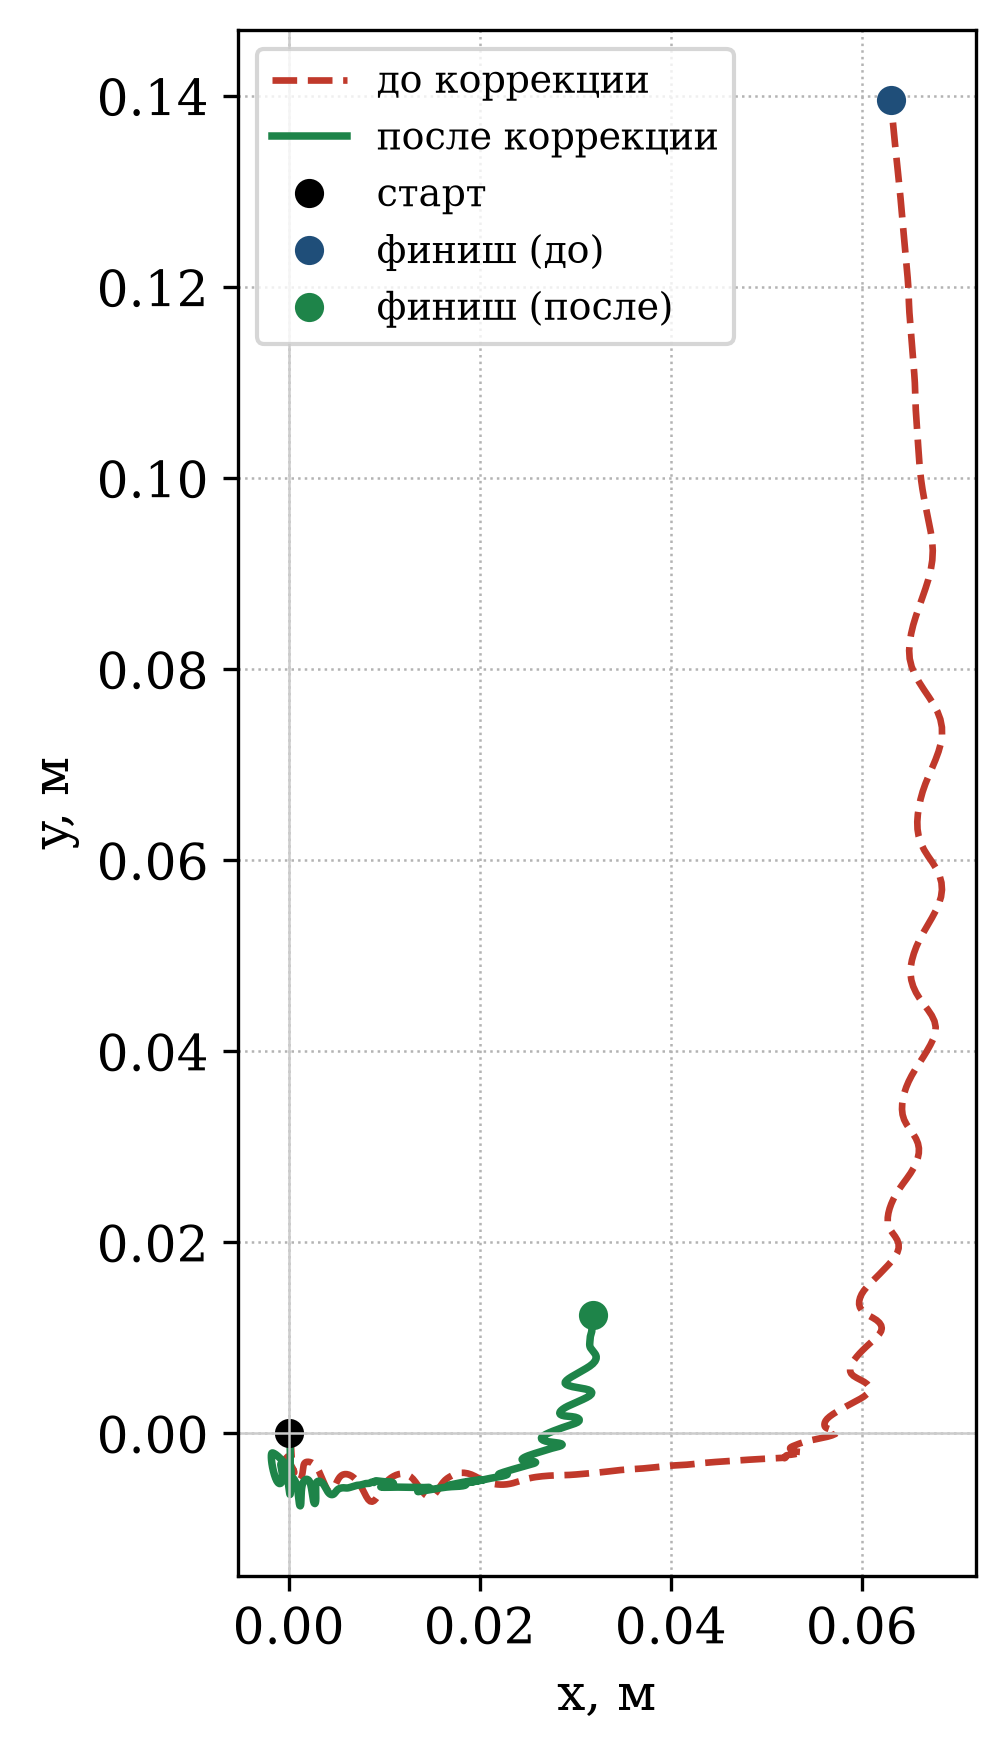
\includegraphics[width=0.72\columnwidth]{figures/fig3_session.png}
  \caption{Траектория покачивания в одной точке до (красная линия) и после (зелёная) коррекции по остановкам}
  \label{fig:real}
\end{figure}

Для версии 0.3.0 значение «после» получено повторной обработкой той же записи: в самой версии 0.3.0 коррекции ещё не было. Ложный уход направлен вдоль оси покачивания, а после остановки линия возвращается к началу. Остаток 0,037~м за 10~с покачивания соответствует постоянной ошибке ускорения меньше 0,001~м/с$^2$; это уровень остаточной неточности калибровки. Коррекция не меняет сырые данные: в \texttt{raw.csv} остаются исходные показания, а исправленная траектория записывается в \texttt{trajectory.csv}; в \texttt{meta.json} сохраняются число исправленных участков, максимальная вычтенная ошибка и сдвиг.

\subsection{Обсуждение}

Полученные числа согласуются с литературой. Ошибка ориентации около $1{,}5$--$2{,}3^\circ$ типична для инерциальных систем без магнитометра~\cite{woodman,zhilin}. Уменьшение ошибки положения в 20 раз при использовании остановок качественно совпадает с результатом~\cite{neto}. Точность 0,08~м за 12-секундный цикл близка к результатам~\cite{neto,kortier}, хотя условия там были другие: лучше датчики и иногда магнитная опора.

Собственные записи подтверждают главный вывод: при покачивании телефона в одной точке основная ошибка~--- не случайный шум, а почти постоянная составляющая ускорения. Коррекция по остановкам убирает её и возвращает линию к началу. Остаток в основном вертикальный: в покое он равен 0,012--0,024~м/с$^2$ и связан с погрешностью масштаба акселерометра.

Ограничения работы: синтетическая модель не учитывает вибрации, нагрев и неровный шаг времени; запись UCI~HAR сделана датчиком на поясе и не имеет истинной траектории; собственные записи проверяют покачивание в одной точке, но не длительные перемещения. Магнитометр не использовался, поэтому курс со временем уходит. Коррекция работает только при наличии остановок; масштаб и перекосы осей гироскопа пока не оцениваются, а плечо датчика относительно точки вращения не компенсируется.

% ============================================================
\section{Заключение}

Собран и проверен конвейер, который по данным акселерометра и гироскопа смартфона оценивает ориентацию кисти и восстанавливает траекторию. Главная проблема инерциальных измерений~--- накопление ошибки при двойном интегрировании. Для борьбы с ней выбраны кватернионное описание ориентации, фильтр Калмана с гейтом акселерометра, детектор остановок, численное интегрирование и коррекция по остановкам.

На синтетической записи ошибка ориентации в модели составила $1{,}48^\circ$, в приложении~--- $2{,}34^\circ$; ошибка положения за 60~с в приложении~--- 0,59~м, после коррекции~--- 0,27~м. На реальной записи UCI~HAR детектор правильно отнёс к покою 97,2\,\% отсчётов и не дал ложных срабатываний при ходьбе. На собственных записях итоговое смещение уменьшилось с 1,423 до 0,071~м и с 0,188 до 0,037~м.

Дальнейшая работа: повторная обработка записей с другими порогами, оценивание масштаба и перекосов осей гироскопа, компенсация плеча датчика, опыты с перемещениями 0,5--1,5~м и эталонным трекером.

% ============================================================
\begin{thebibliography}{99}

\bibitem{woodman} O.~J. Woodman, \textit{An Introduction to Inertial Navigation}, Technical Report No.~696. Cambridge: University of Cambridge Computer Laboratory, 2007, 37~p.

\bibitem{kortier} H.~G. Kortier, V.~I. Sluiter, D. Roetenberg, and P.~H. Veltink, ``Assessment of hand kinematics using inertial and magnetic sensors,'' \textit{Journal of NeuroEngineering and Rehabilitation}, vol.~11, art.~70, 2014, doi: 10.1186/1743-0003-11-70.

\bibitem{shenoy} P. Shenoy, A. Gupta, and S.~K.~M. Varadhan, ``Design and validation of an IMU based full hand kinematic measurement system,'' \textit{IEEE Access}, vol.~10, pp.~93812--93830, 2022, doi: 10.1109/ACCESS.2022.3203186.

\bibitem{pellois} R. Pellois and O. Brüls, ``Human arm motion tracking using IMU measurements in a robotic environment,'' in \textit{Proc. ISMCR 2018 --- 21st Int. Symposium on Measurement and Control in Robotics}, Mons, 2018, 4~p.

\bibitem{miyazaki} T. Miyazaki and Y. Kitazono, ``Study on hand tracking with IMU,'' in \textit{Proc. 7th IIAE Int. Conf. on Industrial Application Engineering}, 2019, pp.~191--194, doi: 10.12792/iciae2019.037.

\bibitem{neto} P. Neto, J.~N. Pires, and A.~P. Moreira, ``3-D position estimation from inertial sensing: minimizing the error from the process of double integration of accelerations,'' in \textit{Proc. IECON 2013 --- 39th Annual Conf. IEEE Industrial Electronics Society}, 2013, pp.~4026--4031, doi: 10.1109/IECON.2013.6699780.

\bibitem{niu} W. Niu, L. Fang, Z. Qi, and D. Guo, ``Small displacement measuring system based on MEMS accelerometer,'' \textit{Mathematical Problems in Engineering}, vol.~2019, art.~3470604, 2019, doi: 10.1155/2019/3470604.

\bibitem{mahony} R. Mahony, T. Hamel, and J.-M. Pflimlin, ``Nonlinear complementary filters on the special orthogonal group,'' \textit{IEEE Transactions on Automatic Control}, vol.~53, no.~5, pp.~1203--1218, 2008, doi: 10.1109/TAC.2008.923738.

\bibitem{zhilin} Д.~Г. Жилин, ``Формирование жестов с использованием инерциальных измерительных модулей и кватернионного описания ориентации,'' \textit{Вестник науки}, №~5 (98), т.~3, с.~1556--1564, 2026.

\bibitem{tedaldi} D. Tedaldi, A. Pretto, and E. Menegatti, ``A robust and easy to implement method for IMU calibration without external equipments,'' in \textit{Proc. IEEE Int. Conf. Robotics and Automation (ICRA)}, 2014, pp.~3042--3049, doi: 10.1109/ICRA.2014.6907297.

\bibitem{zhang} R. Zhang, F. Höflinger, and L.~M. Reindl, ``Calibration of an IMU using 3-D rotation platform,'' \textit{IEEE Sensors Journal}, vol.~14, no.~6, pp.~1778--1787, 2014, doi: 10.1109/JSEN.2014.2303642.

\bibitem{batista} P. Batista, C. Silvestre, P. Oliveira, and B. Cardeira, ``Accelerometer calibration and dynamic bias and gravity estimation: analysis, design, and experimental evaluation,'' \textit{IEEE Transactions on Control Systems Technology}, vol.~19, no.~5, pp.~1128--1137, 2011, doi: 10.1109/TCST.2010.2076321.

\bibitem{epifanov} К.~А. Епифанов, ``Исследование алгоритмов замыкания цикла в лидарной одометрии,'' в сб. \textit{Искусственный интеллект в промышленных, коммерческих, медицинских и финансовых приложениях}, вып.~3. М.: НИТУ «МИСиС», 2025, с.~57--61.

\bibitem{vershinin} К.~А. Вершинин, К.~В. Башурина, ``Непрерывное распознавание языка жестов,'' в сб. \textit{Искусственный интеллект в промышленных, коммерческих, медицинских и финансовых приложениях}, вып.~1. М.: НИТУ «МИСиС», 2023, с.~100--105.

\bibitem{kataev} М.~Ю. Катаев, Н.~Г. Катаева, Р.~А. Чернов, ``Оценка параметров ходьбы человека с помощью двух акселерометров,'' \textit{Доклады Томского государственного университета систем управления и радиоэлектроники (Proceedings of TUSUR)}, т.~24, №~2, с.~51--55, 2021, doi: 10.21293/1818-0442-2021-24-2-51-55.

\bibitem{uci} D. Anguita, A. Ghio, L. Oneto, X. Parra, and J.~L. Reyes-Ortiz, ``A public domain dataset for human activity recognition using smartphones,'' in \textit{Proc. 21st European Symposium on Artificial Neural Networks (ESANN)}, Bruges, 2013, pp.~437--442.

\end{thebibliography}

\end{document}
